%%%%%%%%%%%%%%%%%%%%%%%%%%%%%%%%%%%%%%%%%
% Beamer Presentation
% LaTeX Template
% Version 1.0 (10/11/12)
%
% This template has been downloaded from:
% http://www.LaTeXTemplates.com
%
% License:
% CC BY-NC-SA 3.0 (http://creativecommons.org/licenses/by-nc-sa/3.0/)
%
%%%%%%%%%%%%%%%%%%%%%%%%%%%%%%%%%%%%%%%%%

%----------------------------------------------------------------------------------------
%	PACKAGES AND THEMES
%----------------------------------------------------------------------------------------

\documentclass{beamer}

\mode<presentation> {
\usetheme{Madrid}
}

\usepackage{graphicx} % Allows including images
\usepackage{booktabs} % Allows the use of \toprule, \midrule and \bottomrule in tables

%----------------------------------------------------------------------------------------
%	TITLE PAGE
%----------------------------------------------------------------------------------------

\title[Drought Resiliency]{What Makes Communities Resilient to Drought?} 

\author[DS421]{Dan Blaustein-Rejito \inst{1} \and Ian Bolliger \inst{2} \and Hal Gordon \inst{3} \and Andy Hultgren \inst{3} \and Yang Ju \inst{4} \and Kate Pennington \inst{3} \and Sara Stoudt \inst{5}}
\institute[UC Berkeley] 
{
University of California, Berkeley: DS421 \\
\medskip
\inst{1} GSPP \and \inst{2} ERG \and \inst{3} ARE \and \inst{4} LAEP \and \inst{5} Stats\\ 
\medskip
\textit{danr@berkeley.edu \and bolliger@berkeley.edu \and halgordon@berkeley.edu \and hultgren@berkeley.edu \and yangju90@berkeley.edu \and kate.pennington@berkeley.edu \and sstoudt@berkeley.edu} 
}
\date{\today}

\makeatletter
\def\beamer@andinst{\quad}
\makeatother

\begin{document}

\begin{frame}
\titlepage 
\end{frame}

\begin{frame}
\frametitle{Overview}
\tableofcontents
\end{frame}

%----------------------------------------------------------------------------------------
%	PRESENTATION SLIDES
%----------------------------------------------------------------------------------------

%------------------------------------------------
\section{Introduction}
%------------------------------------------------

\begin{frame}
	\frametitle{Drought}
	\begin{itemize} \itemsep1em
		\item In April 2016 in the United States: 
			\begin{itemize}
				\item 14\% of land was in drought and 34\% was abnormally dry.
				\item 84.3 million people live in drought-affected areas, and 17.5 million live in areas experiencing ”exceptional drought”
			\end{itemize}
		\item In California:
			\begin{itemize}
				\item 90\% of the state is in drought and more than 50\% is in severe to exceptional drought.
				\item 84.3 million people live in drought-affected areas, and 17.5 million live in areas experiencing ”exceptional drought”
			\end{itemize} 
	\end{itemize}
\end{frame}

\begin{frame}
\frametitle{Drought, April 19, 2016}
	\begin{figure}
		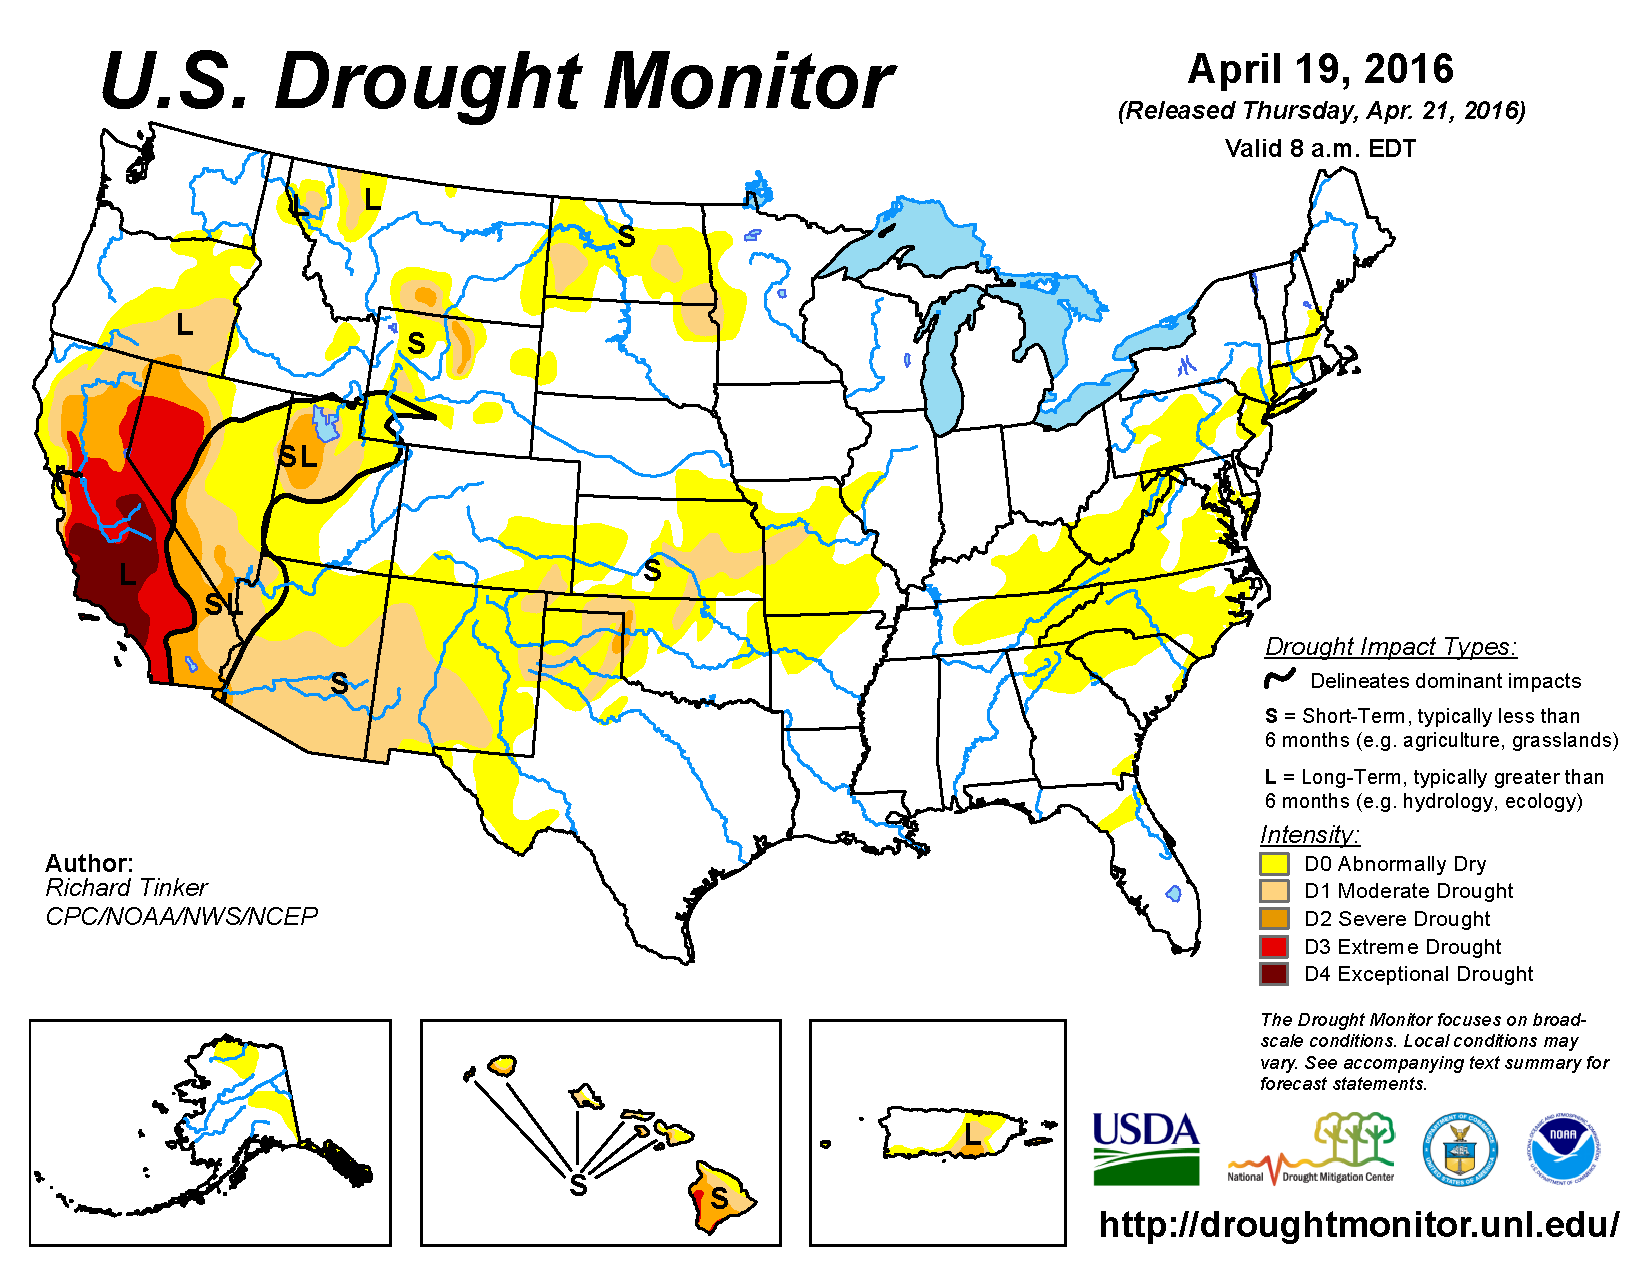
\includegraphics[width=0.8\linewidth]{20160419_usdm}
	\end{figure}	
\end{frame}

\begin{frame}
	\frametitle{Drought}
	\begin{itemize} \itemsep1em
		\item Climate change is likely to increase the length and severity
		\item Resilience, not just risk of drought, will have far reaching implications for welfare changes from climate change.
	\end{itemize}	
\end{frame}

\begin{frame}
	\frametitle{What makes some communities more or less vulnerable to drought?}
	\begin{itemize} \itemsep1em
		\item Welfare impacts not purely determined by severity and duration of drought
		\item We use sensitivity analysis to try to identify some of the salient channels
		\item Two stage analysis:
			\begin{itemize} \item Stage 1: Estimate "vulnerability" = correlation between drought and 'welfare';
			\item Stage 2: Identify predictors of vulnerability \end{itemize}
		\item Unpacking predictors would have important policy implications
	\end{itemize}	
\end{frame}


%------------------------------------------------
\section{Data}
%------------------------------------------------

\begin{frame}
	\frametitle{Stage 1 Data: 2005-2014}
	\textbf{Left Hand Side}
	\begin{itemize}  \itemsep1em
		\item \textbf{US Drought Monitor:}
		\begin{itemize}
			\item Scale from 0-4 updated weekly
			\item we create a 1-year, 3-year, and 5-year measure
		\end{itemize}
	\end{itemize}
	\textbf{Right Hand Side}
	\begin{itemize}
		\item \textbf{Mortality:}
		\begin{itemize}
			\item Annual CDC WONDER database
			\item Over-65 and all-ages
		\end{itemize} 
		\item \textbf{Yields:}
		\begin{itemize}
			\item Annual USDA crop yield
			\item Corn, soybeans, and wheat
		\end{itemize}
		\item \textbf{Employment:}
		\begin{itemize}
			\item United States Bureau of Labor Statistics
		\end{itemize}
	\end{itemize}
\end{frame}

\begin{frame}
	\frametitle{Stage 2 Data}
	\textbf{Left Hand Side}
	\begin{itemize} 
		\item $\hat{\beta}$ from the first stage.
	\end{itemize}
	\textbf{Right Hand Side}
	\begin{itemize}
		\item \textbf{American Community Survey:}
		\begin{itemize}
			\item Annual (2005-2014) survey conducted by US Census
			\item Over 65, Under 5, Race, Ethnicity, Sex, Work in farming or ranching, Household Income, Household water bills
		\end{itemize} 
		\item \textbf{Water Usage:}
		\begin{itemize}
			\item EPA Facility Registry Service
			\item Count of facilities from high water use industries (agriculture, manufacturing and energy) per county
		\end{itemize}
	\end{itemize}
\end{frame}

%------------------------------------------------
\section{Model}
%------------------------------------------------
\subsection{First Stage}

\begin{frame}
	\frametitle{Model}
	\textbf{First Stage Equation}
	\begin{equation}
		y_{i,t} = \beta_{i} D_{i,t} + \alpha_i + \tau_i t + \gamma_{s,t} + \epsilon_{i,t}
	\end{equation}
	Where:
	\begin{itemize}
		\item $D_{i,t}$ refers to the number of days in U.S. Drought Survey bins 2-4 in county $i$ and year $t$
		\item $\alpha_i$ are county fixed effects controlling for time-invariant differences between counties
		\item $\tau_i$ is the coefficient on a county level linear time trend
		\item $\gamma_{s,t}$ are state-by-year fixed effects controlling for state level time trends common across all counties $i \in s$
	\end{itemize}
\end{frame}

%\begin{frame}
%	\frametitle{Model Details}
%	\textbf{First Stage Equation}
%	\begin{itemize}  \itemsep1em
%		\item The state-by-year fixed effects will non-parametrically account for national trends in the outcome of interest as well as state-level trends
%		\item The identifying variation in this model is within-county, annual deviations from the county time trend and from statewide annual average drought levels
%		\item Standard errors will need to be corrected for serial correlation over space and time
%	\end{itemize}
%\end{frame}


%------------------------------------------------
\subsection{Second Stage}

\begin{frame}
	\frametitle{Model}
	\textbf{Second Stage Equation}
	\begin{equation}
		\beta_i = \rho_0 + \boldsymbol{\delta} \mathbf{X}_i + \nu_i
	\end{equation}
	Where:
	\begin{itemize}
		\item $\beta_i$ come from Eq.(1) for a given outcome
		\item $\mathbf{X}_i$ represents a vector of county characteristics such as urban/rural, proportion below age 5 or above age 65, home ownership, median cost of residential water bill
		\item $\boldsymbol{\delta}$ is a vector of the associated coefficients for state level time trends common across all counties $i \in s$
	\end{itemize}
\end{frame}


%\begin{frame}
%	\frametitle{Model Details}
%	\textbf{Second Stage Equation}
%	\begin{itemize}  \itemsep1em
%		\item This regression is cross-sectional and therefore not well identified from a causal perspective
%		\item Model will illustrate how "drought resilience" (a low value of $\beta_i$) covaries with a set of common county socioeconomic characteristics
%		\item We correct OLS standard errors by clustering over space
%	\end{itemize}
%\end{frame}

%------------------------------------------------
\section{Preliminary Results}
%------------------------------------------------

\begin{frame}
	\frametitle{$\beta$ of 3-yr Drought on Corn Yield}
	\begin{figure}
		\includegraphics[width=0.8\linewidth]{"corn 3yr"}
	\end{figure}	
\end{frame}

\begin{frame}
	\frametitle{$\beta$ of 3-yr Drought on Mortality}
	\begin{figure}
		\includegraphics[width=0.8\linewidth]{"mortality 3yr"}
	\end{figure}	
\end{frame}

\begin{frame}
	\frametitle{$\beta$ of 3-yr Drought on Unemployment}
	\begin{figure}
		\includegraphics[width=0.8\linewidth]{"unemp 3yr"}
	\end{figure}	
\end{frame}

\begin{frame}
	\frametitle{Now, look at our Shiny!}
	\begin{figure}
		\includegraphics[height=0.8\textheight]{"shiny"}
	\end{figure}	
\end{frame}
%------------------------------------------------

\begin{frame}
\Huge{\centerline{The End}}
\end{frame}

%----------------------------------------------------------------------------------------

\end{document} 
